\documentclass {article}
\usepackage{graphicx}
\usepackage[utf8]{inputenc}
\graphicspath{ {./images/} }

\title{IT Projekt}
\date{06.05.2019}
\author{Ivaylo Lenkov Ivanov}

\begin{document}

\begin{titlepage}
\maketitle
\end{titlepage}

\section{Einführung}
Für Hauptziel hat dieses Projekt eine virtuelle Umgebung zu bilden und in dieser Umwelt die grundlegende Physik zu simulieren. Die virtuelle Welt ähnelt ein Computerspiel. \\
\begin{figure}[h]
  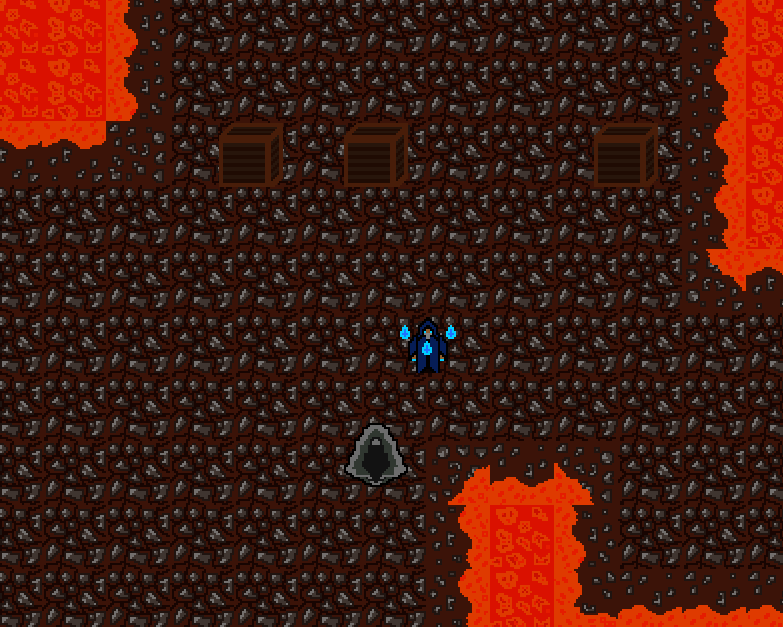
\includegraphics[scale=0.25]{VirtualEnvironment}
\end{figure} \\
Der Benutzer steuert eine virtuelle Figur. \\
\begin{figure}[h]
  
\includegraphics[scale=0.10]{MageCharacter}
\end{figure} \\
Der Avatar kann sich in dem Terrain bewegen und Eiszapfen in jeden Richtung feuern. Die Anfangsszene dem Spiel hat vier Spielobjekte --- drei Kasten und ein Stein.\\
\begin{figure}[h]
  
\includegraphics[scale=15]{Box}
  
\includegraphics[scale=15]{Stone}
\end{figure} \\
Mit den Kisten kann der Anwender interagieren.

\end{document}
